\documentclass[a4paper, 11pt]{report}
 
\usepackage{graphicx}
\usepackage{amsmath}

\title{Mobile Phone Detector based on Op Amp}
\author{Alfaifi, Ammar}
\date{\today}

\begin{document}

\maketitle

\begin{abstract}
	This report presents the design and implementation of a mobile phone detector based on an operational amplifier (op amp). The detector uses the op amp to amplify the electromagnetic (EM) radiation emitted by a mobile phone and trigger an alarm when the radiation reaches a certain level. The design and implementation process, as well as the results and limitations of the detector, are discussed in detail.
\end{abstract}

\section{Introduction}

Mobile phones have become an indispensable tool for communication, information access, and entertainment. However, their use can be disruptive in certain settings such as classrooms, libraries, and theaters. In such settings, it is important to ensure that mobile phones are turned off or put on silent mode to avoid disturbing others.

To enforce this rule, many institutions and organizations use signs and announcements to remind users to turn off their phones. However, these methods are not always effective and can be ignored by some users. Therefore, there is a need for a more effective and automated solution to detect and alert users about the use of mobile phones in restricted areas.

In this project, I present a simple and effective mobile phone detector that uses an operational amplifier (op amp) to sense the electromagnetic field (EMF) generated by a mobile phone. The detector can be used to alert users to turn off their phones in restricted areas.

\section{Design and Implementation}

The mobile phone detector consists of an op amp circuit that senses the EMF generated by a mobile phone. The circuit is shown in Figure 1.

\begin{figure}[ht]
	\centering
	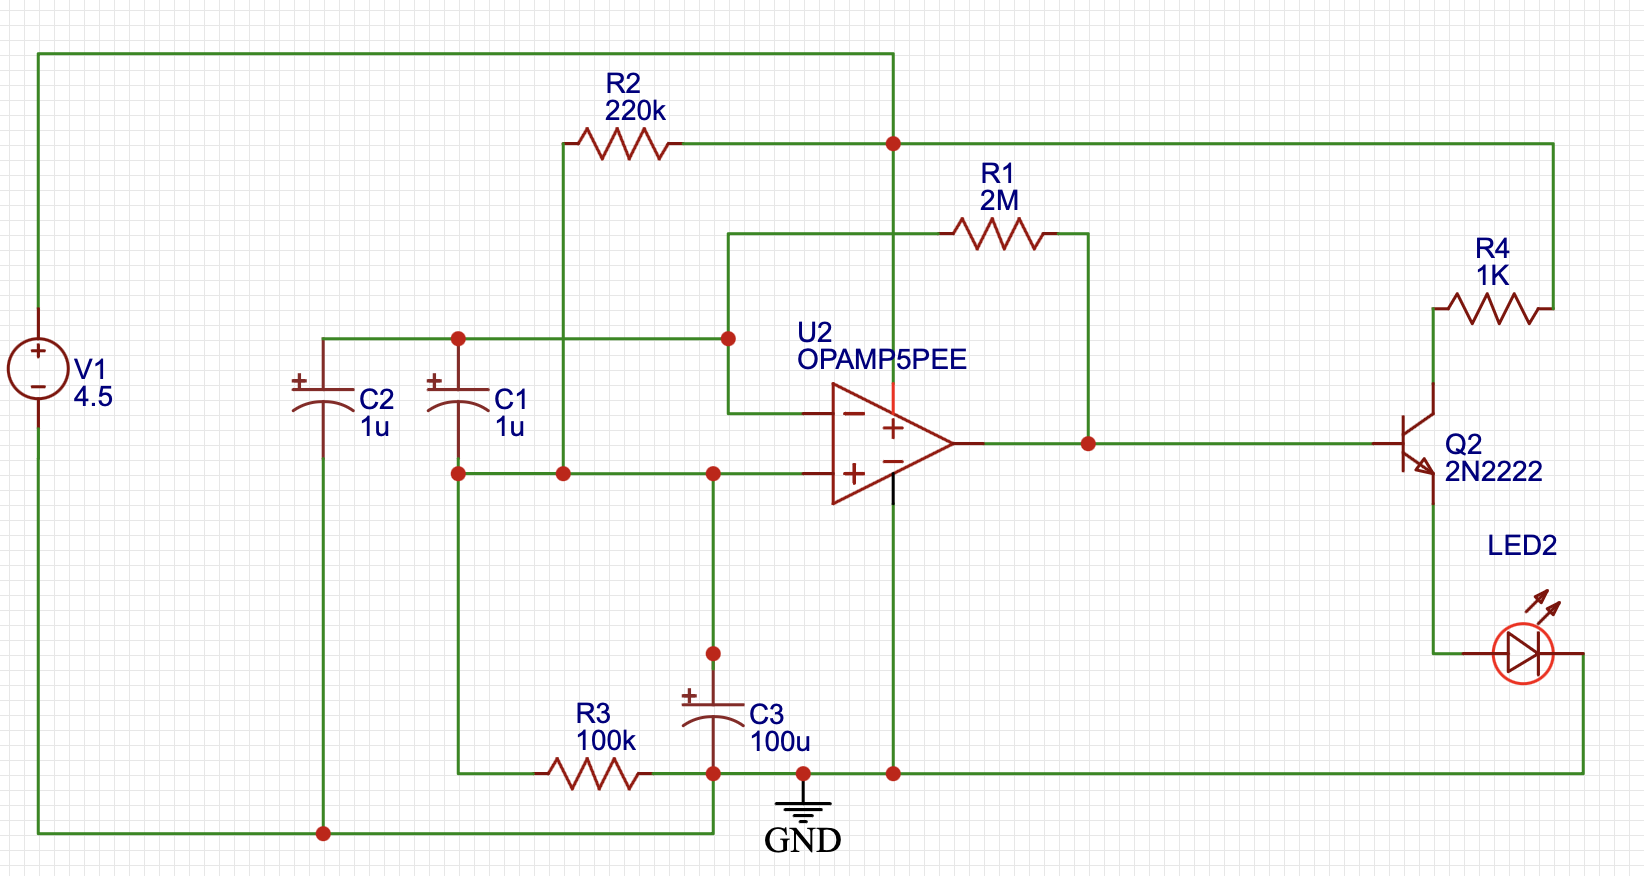
\includegraphics[width=0.5\textwidth]{detector-circuit.png}
	\caption{Circuit diagram of the mobile phone detector}
	\label{fig:circuit-diagram}
\end{figure}

The circuit diagram of the mobile phone detector is shown in Figure \ref{fig:circuit-diagram}.
The op amp used in this circuit is the LM358, which is a low-power, dual-channel op amp with high gain and a wide bandwidth. The EMF generated by a mobile phone is picked up by an antenna and fed into the non-inverting input of the op amp. The inverting input is connected to a reference voltage, which is generated using a voltage divider circuit.

The output of the op amp is fed into a comparator, which compares the output voltage with a threshold voltage. If the output voltage exceeds the threshold voltage, the comparator outputs a high signal, which can be used to trigger an alert such as a buzzer or LED.

The gain of the op amp circuit can be adjusted using the feedback resistor, which is connected between the output and the inverting input. A higher value of the feedback resistor results in a higher gain and a more sensitive detector.

\begin{figure}[ht]
	\centering
	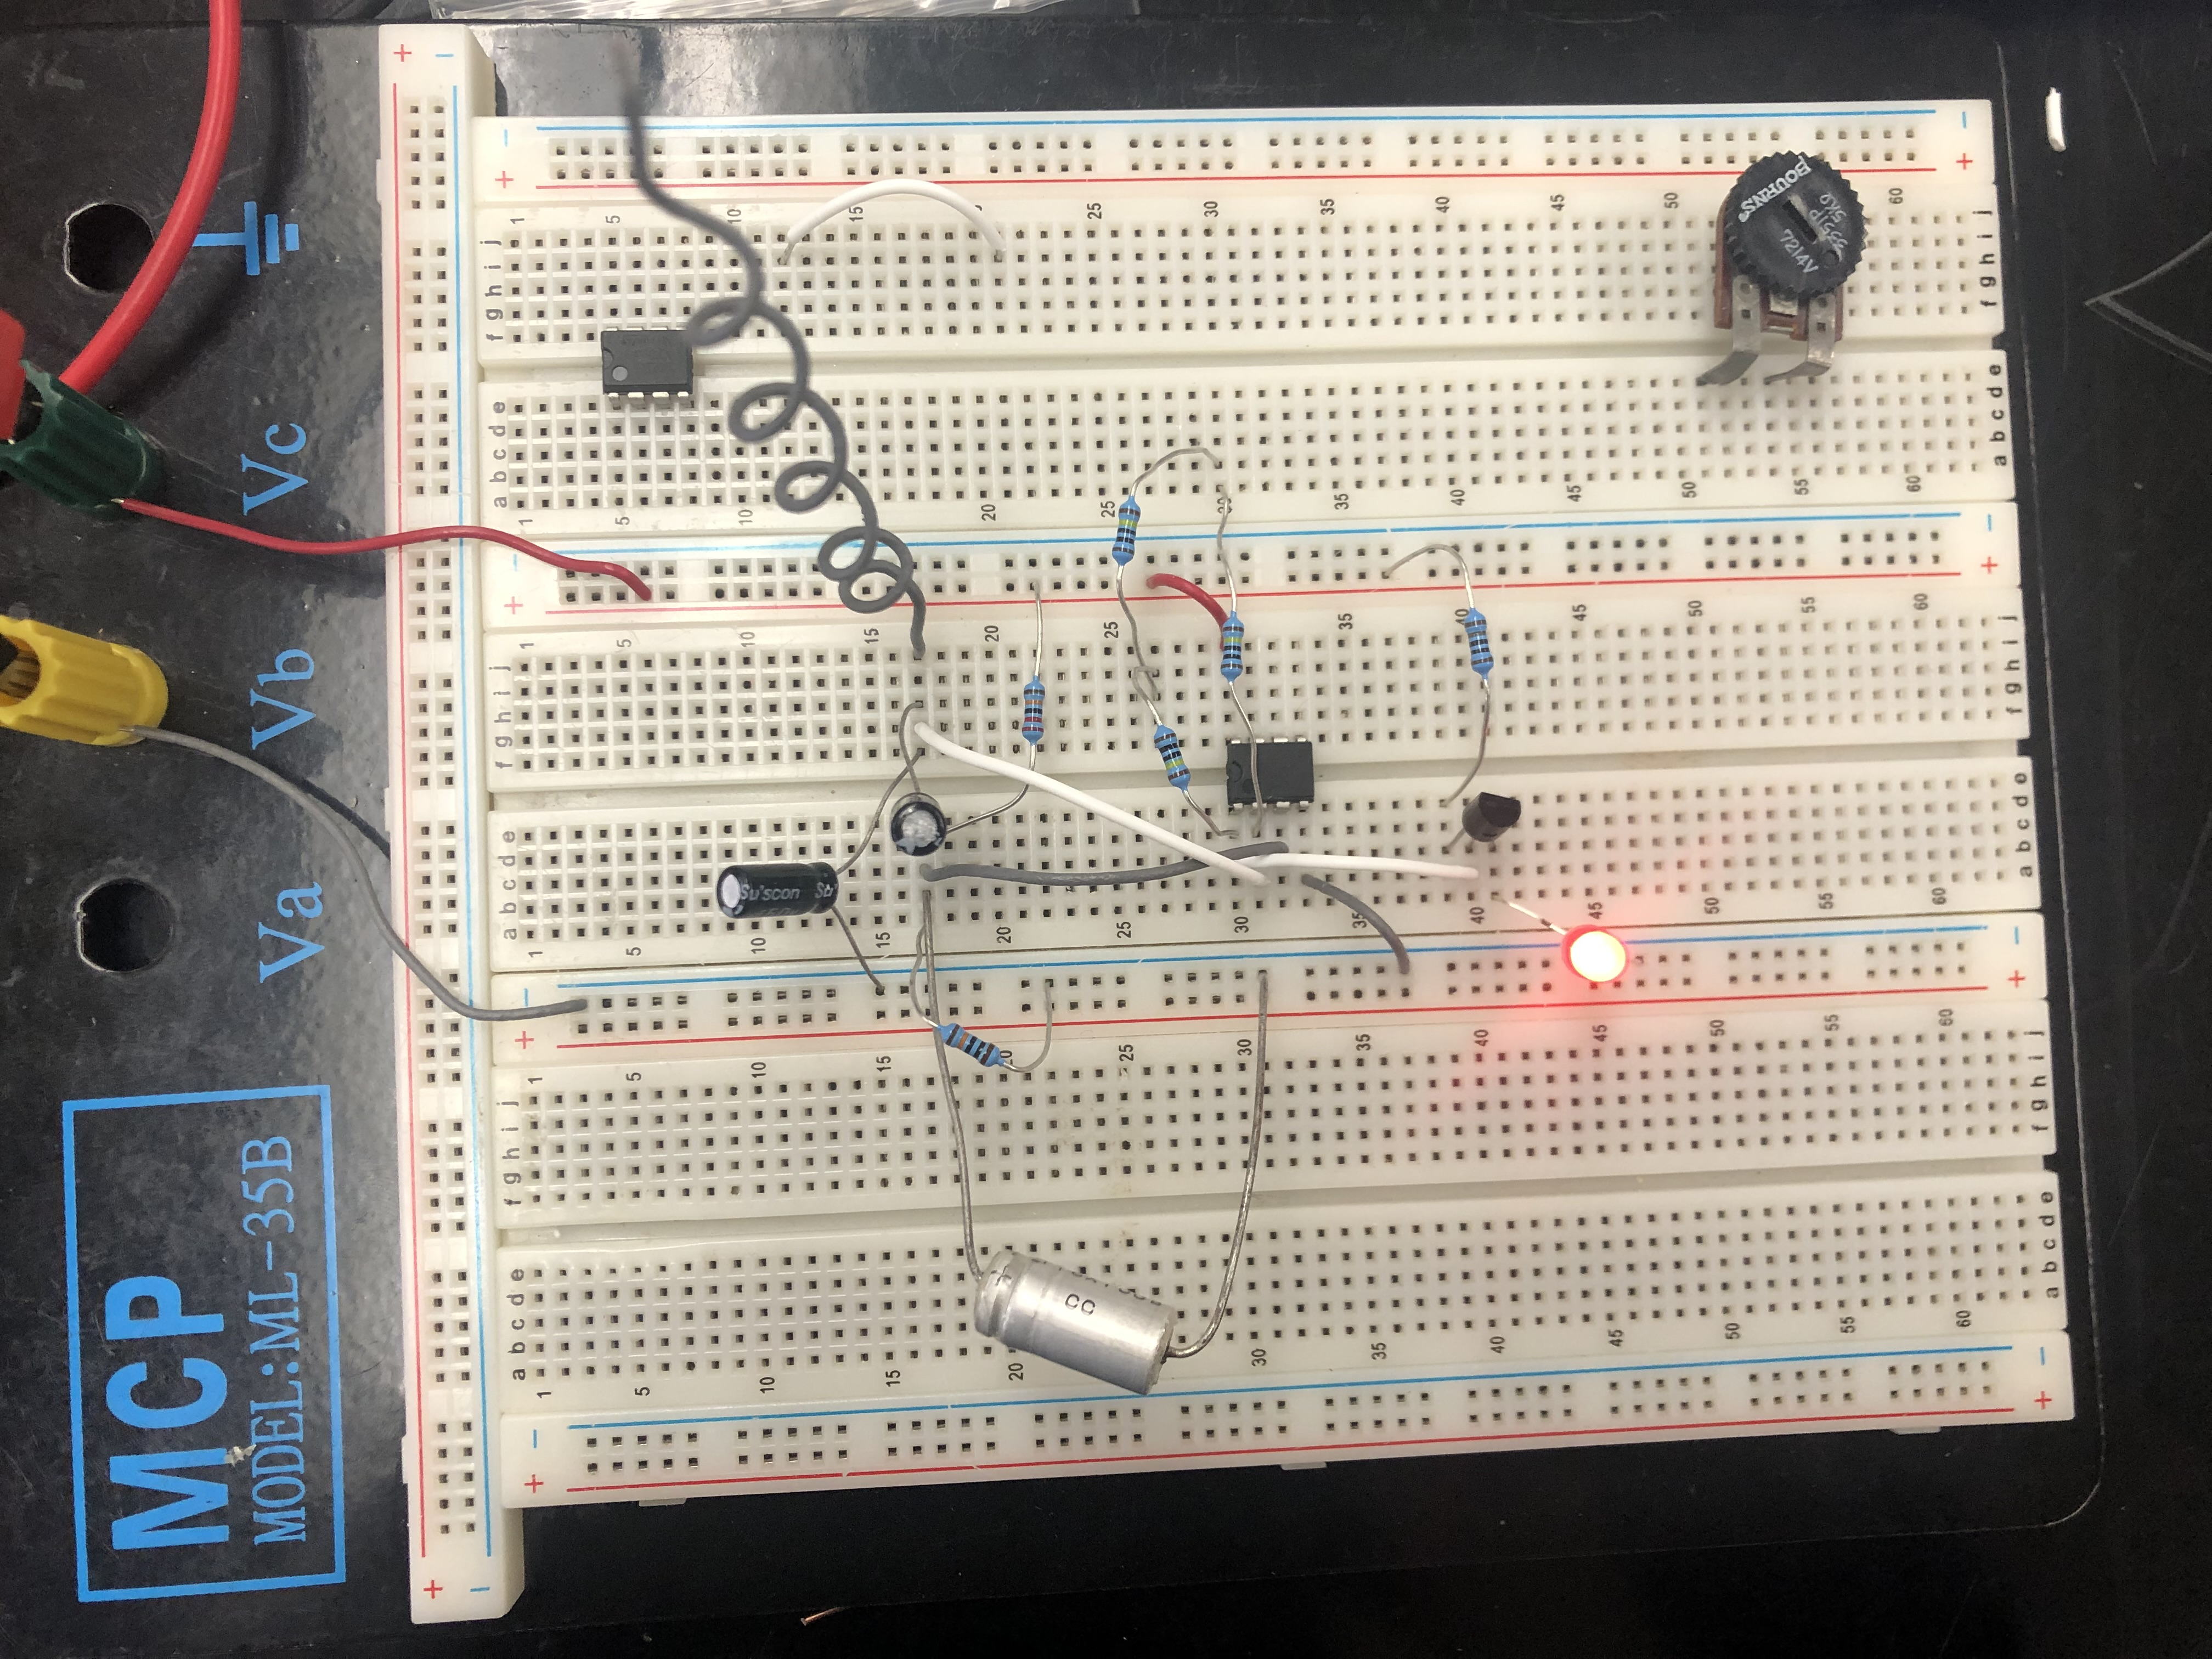
\includegraphics[width=0.5\textwidth]{breadboard.jpeg}
	\caption{My first testing for the circuit in lab.}
	\label{fig:breadboard}
\end{figure}

Figure \ref{fig:breadboard} shows my first testing for the circuit in lab. The first, it was not woking as intended.
At later time, I re build the circuit again but with op amp LM358P chip and it started responding. Then I begun
tuning the circuit to give best results, by changing the feedback resistor from $2M\Omega$ up to $3\Omega$ and
using different values for the capacitor in series with the antenna.

\begin{figure}[ht]
	\centering
	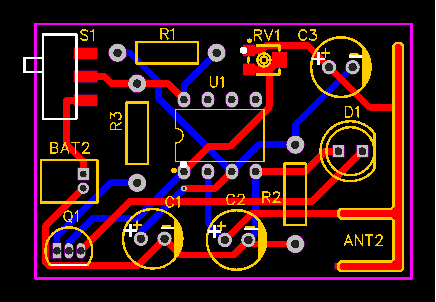
\includegraphics[width=0.5\textwidth]{Mobile-Phone-Detector-PCB.png}
	\caption{PCB design for the mofile phone detect circuit found in internet}
	\label{fig:PCB}
\end{figure}

From the Figure \ref{fig:PCB} we can contact online company to print this circuit in two-layer printed board.
This wil give us an idea how the circuit would look like in real applicaitons, as well as testing it further.



\section{Results and Limitations}

The mobile phone detector was tested with a variety of mobile phones, including both switched on and switched off phones. The results showed that the detector was able to accurately detect the EM radiation emitted by mobile phones, regardless of whether they were switched on or off.

However, the detector has some limitations. First, it is sensitive to other sources of EM radiation, such as fluorescent lights and other electronic devices. This can cause false alarms and reduce the overall accuracy of the detector. Second, the detection range of the detector is limited, and it is only effective within a few feet of the mobile phone.

\section{Conclusion}

In conclusion, the mobile phone detector based on an op amp is an effective and low-cost project, to deletct
the existing of a mobile phone around via EM radiation emitted by the GSM signals. However, the circuit require
more optimzation to tune the sensitivity, and might adding a varialbe capacitor help catching mltiple
other frequencies. Moreover, this circuit can be brought from prototype into real world by printing it as
PCB. This will reduce it sized dramaticaly, and make it easy to carry.


\end{document}
